\documentclass[a4paper,10pt]{article}

\usepackage[margin=3.5cm]{geometry}
\usepackage[format=hang,justification=raggedright,font=it,singlelinecheck=off]{caption}
\usepackage{url,graphicx,paralist,verbatim}

\begin{document}

\title{
  {\small
    Halmstad University course DA4002\\
    Introduction to Algorithms, Data Structures, and Problem Solving\\
  }
  Report Template for Project 1:\\
  Sorting Algorithm Benchmarks
}
\author{
  Student Name One \texttt{<student.email@one>}\\
  Student Name Two \texttt{<student.email@two>}
}
\maketitle



{\itshape

\vfill

\textbf{The report is an essential part of the project work.
It counts for approximately half the points.
The structure of this template should be followed to write your report.}
Most aspects of the report are clearly specified in this template, others are more open-ended and you have to decide how best to structure them to illustrate what you have done and what conclusions you draw from your results.

\vfill

The report should start with a short summary of what you have done (which tasks and which algorithms you have chosen).
Then follows a section on individual algorithm benchmarks, each under its own section heading.
It should contain at least one plot of the runtime in function of problem size.
If you did the second mandatory task, this plot should show the minimum, average, and maximum runtimes.
If you did the third mandatory task, you should add a plot that illustrates how well your empirical measurements match the theoretical complexity.
The plots should be followed by a short text (or bullet list) which
\begin{compactitem}
\item
  specifies references that you used;
\item
  explains where to find your implementation in your code;
\item
  states how to reproduce your plots;
\item
  finishes with a more free-form text about other things you wish to point out, for example where to find test code and what you conclude from the plots.
\end{compactitem}

After the individual algorithms, you should write a section which compares them with each other.
This should include some plots that clearly show how the algorithms in relation to each other, possibly using various ranges on the axes or even logarithmic scale if you think that is the most useful.
The figures should again be followed by a short text that explains how to reproduce the plots with your program, and concludes with another open-ended free-form text.
If you did the first and/or second bonus task, include them in the individual and comparison sections.
If you did the third bonus task, choose your own reporting format such that it properly conveys your insights.

\vfill

\noindent
\bfseries
Do not forget to
\begin{compactitem}
\item
  give the course name, project title, and student names;
\item
  specify references to all the sources you have used, for example links to websites were you found pseudo-code;
\item
  number all the figures and give them short descriptive captions;
\item
  generally include all the information necessary to reproduce your results with your code;
\item
  finish the report with a short overall conclusion.
\end{compactitem}

}
\newpage


\section*{Summary}

This template report illustrates how to present your project results.
It relies on insertion sort and merge sort, which are included in the project assignment.
It does not include a section on bonus task three.
Students who do that bonus task are required to come up with their own structure to clearly demonstrate their findings.



\section*{Individual Algorithms}



\subsection*{Insertion Sort}

\begin{figure}
  \centering
  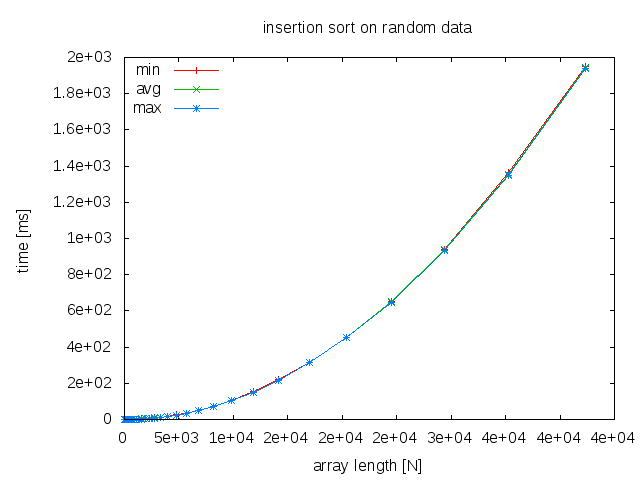
\includegraphics[width=0.7\columnwidth]{examples/isort.png}
  \caption{
    Runtimes of insertion sort on various arrays sizes.
  }\label{fig:isort}
  \vspace{\baselineskip}
  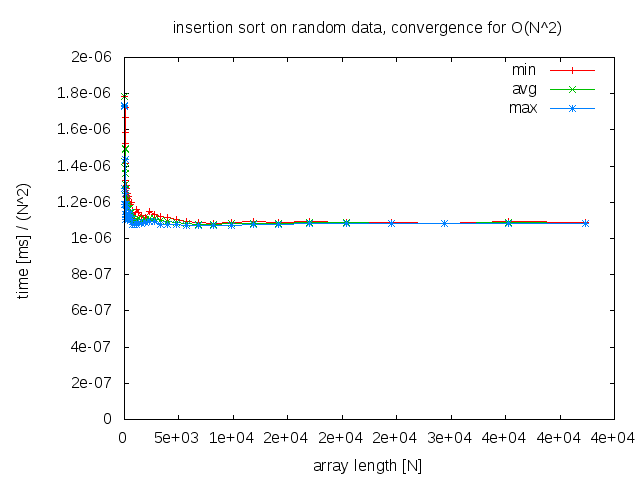
\includegraphics[width=0.7\columnwidth]{examples/isort-N2.png}
  \caption{
    Dividing the measured runtimes of insertion sort by $N^2$ shows a clear convergence to a non-zero value.
  }\label{fig:isort-N2}
\end{figure}

The implementation of insertion sort can be found in the source code \texttt{insertion\--sort\--benchmark.c} in the \texttt{insertion\_sort()} function.
It is based on code examples readily available on the internet, for example on Wikipedia at \url{http://en.wikipedia.org/wiki/Insertion_sort}.

Figure~\ref{fig:isort} shows the minimum, average, and maximum runtimes measured by running insertion sort on five different random arrays that are initialized at the beginning of the \texttt{main()} function\footnote{
  Note that the code included in the project assignment does \emph{not} do this, it is part of mandatory task 1 that you have to do.
  Also note that five runs may not be enough to reduce the noise in the measurements, this is for you to judge based on your measurements.
}.
The benchmark prints the measured times in individual columns, with the minimum, average, and maximum printed in the last three columns.
The figure can be reproduced with the following Gnuplot commands, assuming you have saved the benchmark output into a file called \texttt{data}.

\small\noindent
\verbatiminput{examples/isort.plot}
\normalsize

According to Wikipedia, the theoretical complexity of insertion sort is $O(N^2)$.
Figure~\ref{fig:isort-N2} shows that, if the measured runtimes are divided by $N^2$, the resulting values do converge to a non-zero constant.
This illustrates that theory and practice match each other very closely in this case.
This figure can be reproduced as follows:

\small\noindent
\verbatiminput{examples/isort-N2.plot}
\normalsize



\subsection*{Merge Sort}

\begin{figure}
  \centering
  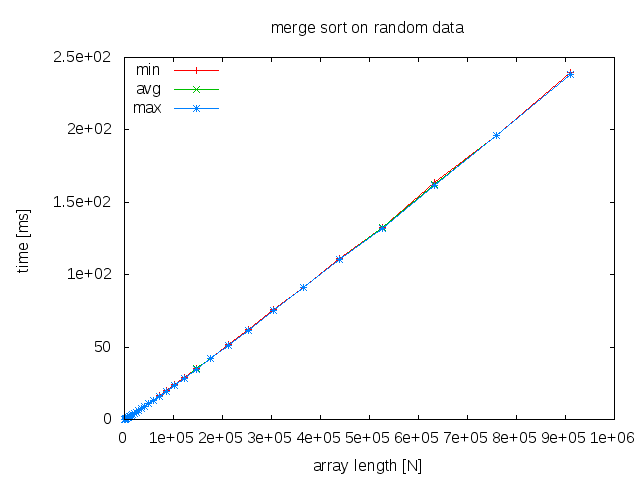
\includegraphics[width=0.7\columnwidth]{examples/msort.png}
  \caption{
    Runtimes of merge sort on various arrays sizes.
  }\label{fig:msort}
  \vspace{\baselineskip}
  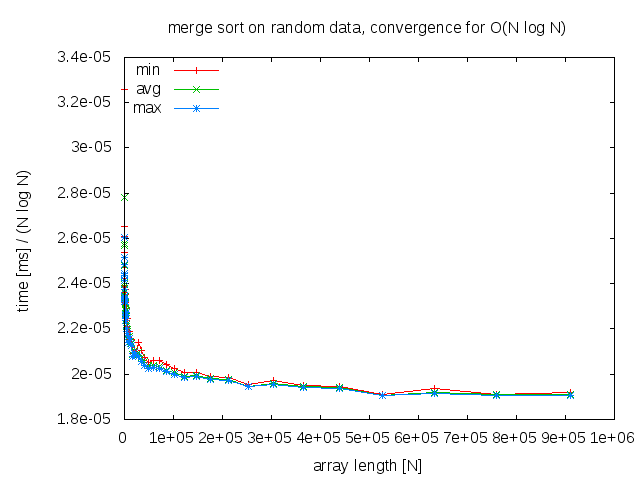
\includegraphics[width=0.7\columnwidth]{examples/msort-NlogN.png}
  \caption{
    Dividing the measured runtimes of insertion sort by $N \log N$ shows a clear convergence to a non-zero value.
  }\label{fig:msort-NlogN}
\end{figure}

The implementation of merge sort can be found in the source code \texttt{merge\--sort\--benchmark.c} in the functions \texttt{merge()}, \texttt{msort\_rec()}, and \texttt{merge\_sort()}.
Examples of merge sort implementations are easily found on the internet, for example on Wikipedia at \url{http://en.wikipedia.org/wiki/Merge_sort}.
In our implementation, the \texttt{merge\_sort()} function is the high-level entry point.
It allocates a temporary array, calls the recursive \texttt{msort\_rec()} which implements the actual algorithm, and then frees the temporary array.
The \texttt{merge()} function takes two arrays (stored within the same memory range but at different indices) that are already sorted, and produces a merged sorted array from them.

Figure~\ref{fig:msort} shows minimum, average, and maximum runtimes over five different runs, similarly to what was done with insertion sort (see the previous section for details).
The figure can be reproduced with the following Gnuplot commands.

\small\noindent
\verbatiminput{examples/msort.plot}
\normalsize

According to Wikipedia, the theoretical complexity of insertion sort is $O(N \log N)$.
Figure~\ref{fig:msort-NlogN} shows that, if the measured runtimes are divided by $N \log N$, the resulting values do converge to a non-zero constant.
This illustrates that theory and practice match each other very closely in this case.
This figure can be reproduced as follows:

\small\noindent
\verbatiminput{examples/msort-NlogN.plot}
\normalsize



\section*{Algorithm Comparison}

\begin{figure}
  \centering
  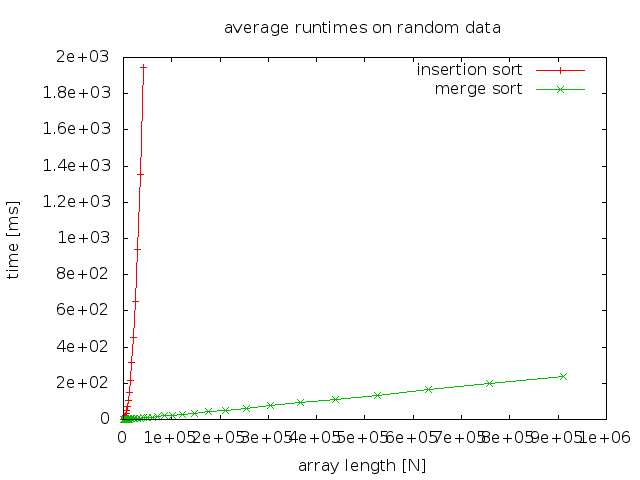
\includegraphics[width=0.7\columnwidth]{examples/isort-msort.png}
  \caption{
    Average runtimes of insertion sort and merge sort on various array sizes.
  }\label{fig:isort-msort}
  \vspace{\baselineskip}
  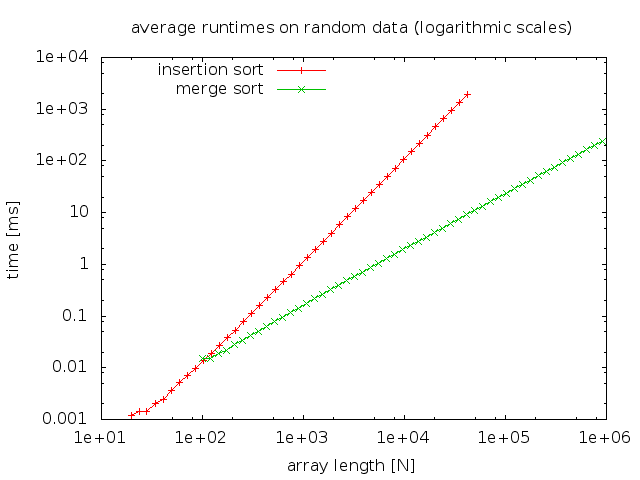
\includegraphics[width=0.7\columnwidth]{examples/isort-msort-logscale.png}
  \caption{
    The same data plotted with logarithmic scales for both $N$ and $T$.
  }\label{fig:isort-msort-logscale}
\end{figure}

Figure~\ref{fig:isort-msort} shows the average runtime measurements for all implemented algorithms.
It can be produced with the following Gnuplot commands, assuming that the insertion sort runtime data is stored in a file called \texttt{isort.data} and the merge sort data in \texttt{msort.data}:

\small\noindent
\verbatiminput{examples/isort-msort.plot}
\normalsize

To better separate the slow-growing from the fast-growing curves, Figure~\ref{fig:isort-msort-logscale} shows the same data on logarithmic scales.
It can be produced with the following commands:

\small\noindent
\verbatiminput{examples/isort-msort-logscale.plot}
\normalsize

These figures clearly show that merge sort is orders of magnitude faster than insertion sort on the larger problem sizes.
This is as expected, given that merge sort has a lower runtime complexity of $O(N \log N)$ whereas insertion sort is $O(N^2)$ which grows much faster.
On the other hand, both algorithms take approximately the same time for $N\approx 100$.
It can be expected that for smaller $N$, insertion sort would actually run faster than merge sort.



\section*{Conclusion}

The runtime measurements performed with our benchmark programs for insertion sort and merge sort shows a good match between theoretical and empirical runtime complexity on random data.
In our measurements, the minimum, maximum, and average values were close together, so the average was chosen in the comparison section to represent each algorithm.
If more noise is present, it can be expected that using the minimum would be the best representative.


\end{document}
